

\tikzset{every picture/.style={line width=0.75pt}} %set default line width to 0.75pt        

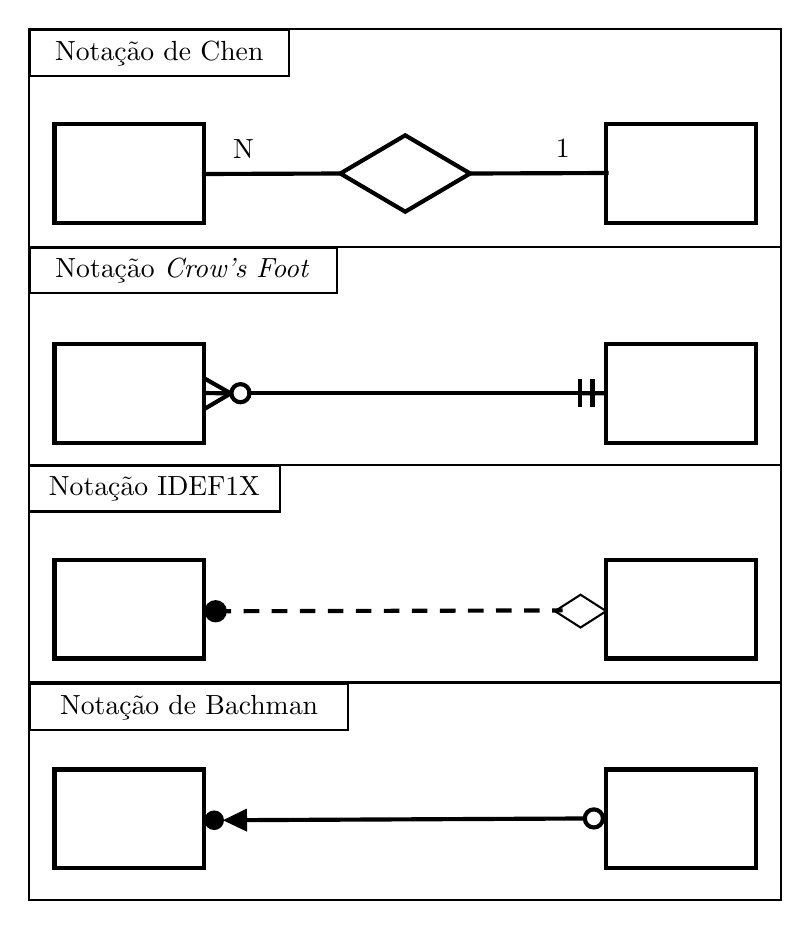
\begin{tikzpicture}[x=0.75pt,y=0.75pt,yscale=-1,xscale=1]
%uncomment if require: \path (0,525.1999969482422); %set diagram left start at 0, and has height of 525.1999969482422

%Shape: Diamond [id:dp5322960225109352] 
\draw  [line width=1.5]  (237.4,69.56) -- (268.68,87.96) -- (237.4,106.36) -- (206.13,87.96) -- cycle ;
%Shape: Rectangle [id:dp3461472448170224] 
\draw  [line width=1.5]  (68.4,64.28) -- (140.51,64.28) -- (140.51,111.63) -- (68.4,111.63) -- cycle ;
%Shape: Rectangle [id:dp4599906974909618] 
\draw  [line width=1.5]  (334.29,64.28) -- (406.4,64.28) -- (406.4,111.63) -- (334.29,111.63) -- cycle ;
%Straight Lines [id:da7414062696338117] 
\draw [line width=1.5]    (139.4,88.2) -- (206.13,87.96) ;


%Straight Lines [id:da23026930680447055] 
\draw [line width=1.5]    (268.68,87.96) -- (335.4,87.72) ;


%Shape: Rectangle [id:dp8341037786755543] 
\draw  [line width=1.5]  (68.4,274.28) -- (140.51,274.28) -- (140.51,321.63) -- (68.4,321.63) -- cycle ;
%Shape: Rectangle [id:dp31798113588606736] 
\draw  [line width=1.5]  (334.29,274.28) -- (406.4,274.28) -- (406.4,321.63) -- (334.29,321.63) -- cycle ;
%Straight Lines [id:da598335399198086] 
\draw [line width=1.5]  [dash pattern={on 5.63pt off 4.5pt}]  (146.07,298.86) -- (313.2,298.46) ;

\draw [shift={(146.07,298.86)}, rotate = 359.86] [color={rgb, 255:red, 0; green, 0; blue, 0 }  ][fill={rgb, 255:red, 0; green, 0; blue, 0 }  ][line width=1.5]      (0, 0) circle [x radius= 4.36, y radius= 4.36]   ;
%Shape: Diamond [id:dp6276925099003055] 
\draw   (321.88,290.9) -- (334.22,298.8) -- (321.88,306.7) -- (309.53,298.8) -- cycle ;
%Shape: Rectangle [id:dp5987534833309474] 
\draw  [line width=1.5]  (68.4,375.13) -- (140.51,375.13) -- (140.51,422.48) -- (68.4,422.48) -- cycle ;
%Shape: Rectangle [id:dp923966100487589] 
\draw  [line width=1.5]  (334.29,375.13) -- (406.4,375.13) -- (406.4,422.48) -- (334.29,422.48) -- cycle ;
%Straight Lines [id:da9071541568075199] 
\draw [line width=1.5]    (152.57,399.54) -- (324.93,398.7) ;
\draw [shift={(328.29,398.68)}, rotate = 359.72] [color={rgb, 255:red, 0; green, 0; blue, 0 }  ][line width=1.5]      (0, 0) circle [x radius= 4.36, y radius= 4.36]   ;
\draw [shift={(149.57,399.55)}, rotate = 359.72] [fill={rgb, 255:red, 0; green, 0; blue, 0 }  ][line width=1.5]  [draw opacity=0] (11.61,-5.58) -- (0,0) -- (11.61,5.58) -- cycle    ;
%Shape: Circle [id:dp892362699268519] 
\draw  [fill={rgb, 255:red, 0; green, 0; blue, 0 }  ,fill opacity=1 ] (141.14,399.55) .. controls (141.14,397.22) and (143.03,395.34) .. (145.35,395.34) .. controls (147.68,395.34) and (149.57,397.22) .. (149.57,399.55) .. controls (149.57,401.88) and (147.68,403.76) .. (145.35,403.76) .. controls (143.03,403.76) and (141.14,401.88) .. (141.14,399.55) -- cycle ;
%Shape: Rectangle [id:dp4762144955627674] 
\draw  [line width=1.5]  (68.4,170.28) -- (140.51,170.28) -- (140.51,217.63) -- (68.4,217.63) -- cycle ;
%Shape: Rectangle [id:dp13462140003846312] 
\draw  [line width=1.5]  (334.29,170.28) -- (406.4,170.28) -- (406.4,217.63) -- (334.29,217.63) -- cycle ;
%Straight Lines [id:da4675675836280293] 
\draw [line width=1.5]    (161.38,193.8) -- (321.62,193.8) ;
\draw [shift={(321.62,193.8)}, rotate = 180] [color={rgb, 255:red, 0; green, 0; blue, 0 }  ][line width=1.5]    (0,6.71) -- (0,-6.71)(-6.03,6.71) -- (-6.03,-6.71)   ;
\draw [shift={(158.02,193.8)}, rotate = 0] [color={rgb, 255:red, 0; green, 0; blue, 0 }  ][line width=1.5]      (0, 0) circle [x radius= 4.36, y radius= 4.36]   ;
%Straight Lines [id:da891422235378027] 
\draw [line width=1.5]    (153.37,193.9) -- (140.68,193.72) ;


%Straight Lines [id:da6698767212146683] 
\draw [line width=1.5]    (153.37,193.9) -- (141.03,186.9) ;


%Straight Lines [id:da699977038647627] 
\draw [line width=1.5]    (153.37,193.9) -- (140.37,201.57) ;


%Straight Lines [id:da3688505022442643] 
\draw [line width=1.5]    (321.62,193.8) -- (334.2,193.87) ;


%Shape: Rectangle [id:dp6749930493862317] 
\draw   (56,18.2) -- (418.3,18.2) -- (418.3,123.2) -- (56,123.2) -- cycle ;
%Shape: Rectangle [id:dp8540602211016675] 
\draw   (56,123.2) -- (418.3,123.2) -- (418.3,228.2) -- (56,228.2) -- cycle ;
%Shape: Rectangle [id:dp5100324952449573] 
\draw   (56,228.2) -- (418.3,228.2) -- (418.3,333.2) -- (56,333.2) -- cycle ;
%Shape: Rectangle [id:dp922444451928095] 
\draw   (56,333.2) -- (418.3,333.2) -- (418.3,438.2) -- (56,438.2) -- cycle ;

% Text Node
\draw (159.5,76) node  [align=left] {N};
% Text Node
\draw (313.3,76) node  [align=left] {1};
% Text Node
\draw    (56.4,19) -- (181.4,19) -- (181.4,41) -- (56.4,41) -- cycle  ;
\draw (118.9,30) node  [align=left] {Notação de Chen};
% Text Node
\draw    (56.07,228.82) -- (177.07,228.82) -- (177.07,250.82) -- (56.07,250.82) -- cycle  ;
\draw (116.57,239.82) node  [align=left] {Notação IDEF1X};
% Text Node
\draw    (56.73,334.01) -- (209.73,334.01) -- (209.73,356.01) -- (56.73,356.01) -- cycle  ;
\draw (133.23,345.01) node  [align=left] {Notação de Bachman};
% Text Node
\draw    (56.4,123.67) -- (204.4,123.67) -- (204.4,145.67) -- (56.4,145.67) -- cycle  ;
\draw (130.4,134.67) node  [align=left] {Notação \textit{Crow's Foot}};


\end{tikzpicture}
